\documentclass[]{article}
\usepackage[margin=0.5in]{geometry}
\usepackage{amsthm}
\usepackage{mathtools}
\usepackage{amsfonts}
\usepackage{tikz}
\usetikzlibrary{matrix}

\newtheorem{definition}{Definition}[section]
\newtheorem{theorem}{Theorem}[section]
\newtheorem{lemma}[theorem]{Lemma}



%opening
\title{Verifying Featured Transition Systems using Variability Parity Games}
\author{Sjef van Loo}

\begin{document}

\maketitle

\section{Definitions}
\subsection{Transition systems}
Similar to \cite{Classen2013FeaturedTS}.

\begin{definition}An LTS is a tuple $M = (S, Act, trans, s_0)$, where:
	\begin{itemize}
		\item $S$ is a set of states,
		\item $Act$ a set of actions,
		\item $trans \subseteq S \times Act \times S$ is the transition relation with $(s,a,s') \in trans$ denoted by $s \xrightarrow a s'$,
		\item $s_0 \in S$ is the initial state.
	\end{itemize}
\end{definition}

\begin{definition}An FTS is a tuple $M = (S, Act, trans, s_0, N, P, \gamma)$, where:
	\begin{itemize}
		\item $S, Act, trans, s_0$ are defined as in an LTS,
		\item $N$ is a set of features,
		\item $P \subseteq \mathcal{P}(N)$ is a set of products, ie. feature assignments, that are valid,
		\item $\gamma : trans \rightarrow \mathbb{B}(N)$ is a total function, labelling each transition with a Boolean expression over the features. A product $p \in \mathcal{P}(N)$ satisfying the Boolean expression of transition $t$ is denoted by $p \models \gamma(t)$, $\gamma(t)(p) = 1$ or $p \in [\![\gamma(t)]\!]$. 
		
		A transition $s \xrightarrow a s'$ and $\gamma((s,a,s')) = f$ is denoted by $s \xrightarrow {a / f} s'$. 
	\end{itemize}
\end{definition}

\begin{definition}
	The projection of an FTS $M$ to a product $p \in P$, noted $M_{|p}$, is the LTS $M'=(S,Act,trans', s_0)$, where $trans' = \{t \in trans\ |\ p \models \gamma(t)\}$.
\end{definition}

\begin{definition}\cite{Bradfield2018}
	A modal $\mu$-calculus formula over the set of actions $\mathcal{A}$ and a set of variables $\mathcal{X}$ is defined by
	\[ \varphi = \top\ |\ \bot\ |\ X\ |\ \varphi \vee \varphi\ |\ \varphi \wedge \varphi\ |\ \langle a \rangle \varphi\ |\ [a]\varphi\ |\ \mu X.\varphi\ |\ \nu X.\varphi \]
	with $a \in \mathcal{A}$ and $X \in \mathcal{X}$. 
	
	
	No negations in the language because negations can be pushed inside to the propositions, ie. the $\top$ and $\bot$ elements..
\end{definition}
A fixed point formula $\varphi$ with variable $X$ can be unfolded; the occurrences of $X$ are replaced by $\varphi$. A fixed point formula is equivalent to its unfolding, ie. $\mu X. \varphi$ is equivalent to $\mu X. \varphi[X:=\mu X. \varphi]$. \cite{Bradfield2018}
\section{Goal}
Similar to \cite{inproceedings}.

Given an FTS $M = (S, Act, trans, s_0, N, P, \gamma)$ and a modal $\mu$-calculus formula $\varphi$ we want to find the set $P_s \subseteq P$ such that:
\begin{itemize}
	\item for every $p \in P_s$ we have $M_{|p} \models \varphi$,
	\item for every $p \in P \backslash P_s$ we have $M_{|p} \not\models \varphi$.
\end{itemize}
A counterexample for every $p \in P \backslash P_s$ is preferred.

If $P_s = P$, ie. all products satisfy $\varphi$, we write $M \models \varphi$.

\section{Parity Games}
\subsection{Parity games}
\begin{definition}
	A parity game (PG) is a tuple $G = (V, V_0, V_1, E, \rho)$, where:
	\begin{itemize}
		\item $V = V_0 \cup V_1$ and $V_0 \cap V_1 = \emptyset$,
		\item $V_0$ is the set of vertices owned by player $0$,
		\item $V_1$ is the set of vertices owned by player $1$, 
		\item $E \subseteq V \times V$ is the edge relation,
		\item $\rho :  V \rightarrow \mathbb{N}$ is a priority assignment.
	\end{itemize}
\end{definition}
\subsection{Featured parity games}
\begin{definition}
	A featured parity game (FPG) is a tuple $G = (V,V_0, V_1, E, \rho, N, P, \gamma, v_0)$, where:
	\begin{itemize}
		\item $V = V_0 \cup V_1$ and $V_0 \cap V_1 = \emptyset$,
		\item $V_0$ is the set of vertices owned by player $0$,
		\item $V_1$ is the set of vertices owned by player $1$, 
		\item $E \subseteq V \times V$ is the edge relation,
		\item $\rho :  V \rightarrow \mathbb{N}$ is a priority assignment,
		\item $N$ is a set of features,
		\item $P$ is a set of products
		\item $\gamma : E \rightarrow \mathbb{B}(N)$ is a total function, labelling each edge with a Boolean expression over the features,
		\item $v_0 \in V$ is a starting vertex.
	\end{itemize}
\end{definition}
An FPG is played by player $0$ and $1$. A FPG is played for a specific product $p \in P$, the game starts by placing a token on a vertex $v \in V$. When the token is on vertex $v \in V$ that is owned by player $\alpha \in \{0,1\}$, ie. $v \in V_\alpha$, then player $\alpha$ can move the token to another vertex $w$ such that $(v,w) \in E$ and $p \models \gamma(v,w)$.

For a $p \in P$ we have winnings sets $W_0^p \subseteq V$ and $W_1^p \subseteq V$.
\begin{definition}
The projection from FPG $G^F = (V^F,V_0^F, V_1^F, E^F, \rho^F, N, P, \gamma, v_0)$ to a product $p \in P$, noted $G^F_{|p}$, is the parity game $(V,V_0,V_1, E, \rho)$ where:
\begin{itemize}	
	\item $(V,E)$ is the subgraph of $(V^F,E')$ that is reachable from $v_0 \in V^F$. With $E' = \{ e \in E^F| p \models \gamma(e) \}$,
	\item $V_0 = V_0^F \cap V$,
	\item $V_1 = V_1^F \cap V$,
	\item $\rho(v) = \rho^F(v)$ for all $v \in V$.
\end{itemize}
\end{definition}
\subsection{Variability parity games}
\begin{definition}
	A variability parity game (VPG) is a tuple $G = (V,V_0, V_1, E, \rho, \mathfrak{C}, \theta)$, where:
	\begin{itemize}
		\item $V = V_0 \cup V_1$ and $V_0 \cap V_1 = \emptyset$,
		\item $V_0$ is the set of vertices owned by player $0$,
		\item $V_1$ is the set of vertices owned by player $1$, 
		\item $E \subseteq V \times V$ is the edge relation; we assume that $E$ is total, i.e. for all $v\in V$ there is some $w \in V$ such that $(v,w) \in E$,
		\item $\rho :  V \rightarrow \mathbb{N}$ is a priority assignment,
		\item $\mathfrak{C}$ is a finite set of configurations,
		\item $\theta : E \rightarrow \mathcal{P}(\mathfrak{C})\ \backslash\ \{0\}$ is the configuration mapping, satisfying for all $v \in V$, $\bigcup\{\theta(v,w)|(v,w) \in E\} = \mathfrak{C}$.
	\end{itemize}
\end{definition}
A VPG is played by player $0$ and $1$. A VPG is played for a specific $c \in \mathfrak{C}$, the game starts by placing a token on a vertex $v \in V$. When the token is on vertex $v \in V$ that is owned by player $\alpha \in  \{0,1\}$, ie. $v \in V_\alpha$, then player $\alpha$ can move the token to another vertex $w$ such that $(v,w) \in E$ and $c \in \theta(v,w)$.

For a $c \in \mathfrak{C}$ we have winnings sets $W_0^c \subseteq V$ and $W_1^c \subseteq V$.

\subsection{Relations}
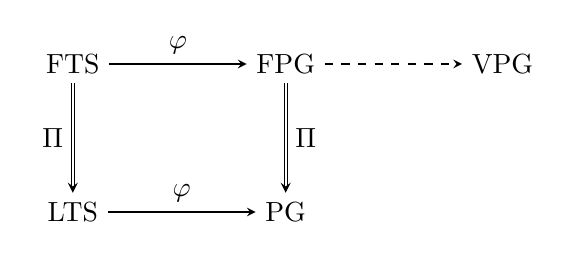
\begin{tikzpicture}
\matrix (m) [matrix of math nodes,row sep=4em,column sep=5em,minimum width=2em]
{
	\text{FTS} & \text{FPG} & \text{VPG} \\
	\text{LTS} & \text{PG} \\};
\path[-stealth]
(m-1-1) edge [double] node [left] {$\Pi$} (m-2-1)
edge node [above] {$\varphi$} (m-1-2)
(m-2-1.east|-m-2-2) edge node [above] {$\varphi$} (m-2-2)
(m-1-2) edge [double] node [right] {$\Pi$} (m-2-2)
edge [dashed] (m-1-3);
\end{tikzpicture}
\subsection{Creating parity games}
\begin{definition}\cite{Bradfield2018}
	LTS2PG($M, \varphi$) converts LTS $M = (S, Act, trans, s_0)$ and formula $\varphi$ to a PG $(V, V_0, V_1, E, \rho)$.
	
	A vertex in the parity game is represented by a pair $(s, \psi)$ where $s \in S$ and $\psi$ is a modal $\mu$-calculus formula.
	
	We create the parity game with the smallest sets $V, V_0, V_1, E$ such that:
	\begin{itemize}
		\item $V = V_0 \cup V_1$,
		\item $V_0 \cap V_1 = \emptyset$, 
		\item $(s_0, \varphi) \in V$,
		\item for every $v = (s, \psi) \in V$ we have:
		\begin{itemize}
			\item If $\psi = \top$ then $v \in V_1$.
			\item If $\psi = \bot$ then $v \in V_0$.
			\item If $\psi = \psi_1 \vee \psi_2$ then:
				\subitem $v \in V_0$,
				\subitem $(s, \psi_1) \in V$,
				\subitem $(s, \psi_2) \in V$,
				\subitem $(v, (s,\psi_1)) \in E$ and
				\subitem $(v, (s,\psi_2)) \in E$.
			\item If $\psi = \psi_1 \wedge \psi_2$ then:
				\subitem $v \in V_1$,
				\subitem $(s, \psi_1) \in V$,
				\subitem $(s, \psi_2) \in V$,
				\subitem $(v, (s,\psi_1)) \in E$ and
				\subitem $(v, (s,\psi_2)) \in E$.
			\item If $\psi = \langle a \rangle \psi_1$ then $v \in V_0$ and for every $s \xrightarrow{ a} s'$ we have $(s', \psi_1) \in V$ and $(v, (s', \psi_1)) \in E$.
			\item If $\psi = [ a ] \psi_1$ then $v \in V_1$ and for every $s \xrightarrow{ a} s'$ we have $(s', \psi_1) \in V$ and $(v, (s', \psi_1)) \in E$.
			\item If $\psi = \mu X. \psi_1$ then $(v, (s, \psi_1(\mu X. \psi_1[X:=\mu X. \psi_1]))) \in E$.
			\item If $\psi = \nu X. \psi_1$ then $(v, (s, \psi_1(\nu X. \psi_1[X:=\mu X. \psi_1]))) \in E$.
		\end{itemize}
	\end{itemize}

Finally we have $\rho(s, \psi) = \begin{cases}
2 \lfloor adepth(X) / 2 \rfloor & \text{if } \psi = \nu X. \psi'\\
2 \lfloor adepth(X) / 2 \rfloor + 1 & \text{if } \psi = \mu X. \psi'\\
0 & \text{otherwise}
\end{cases}$
\end{definition}

\begin{definition}
	FTS2FPG($M, \varphi$) converts FTS $M = (S, Act, trans, s_0, N, P, \gamma)$ and formula $\varphi$ to FPG $(V, V_0, V_1, E, \rho, N, P, \gamma', v_0)$.
	
	We have $(V, V_0, V_1, E, \rho)$ = LTS2PG($(S, Act, trans, s_0), \varphi$), $v_0 = (s_0, \varphi)$ and
	\[ \gamma'((s, \psi),(s', \psi')) = \begin{cases}
	\gamma(s,a,s') & \text{if }\psi = \langle a \rangle \psi'\text{ or }\psi = [a]\psi' \\
	\top & \text{otherwise}
	\end{cases}\]
\end{definition}

\begin{definition}
	FPG2VPG($G^F$) converts FPG $G^F = (V^F, V_0^F, V_1^F, E^F, \rho^F, N, P, \gamma, v_0)$ to VPG $G = (V, V_0, V_1, E, \rho, \mathfrak{C}, \theta)$.
	
	Let $P$ be defined as  $\{p_0, p_1, \dots, p_m\}$, we define $\mathfrak{C} = \{c_0, c_1, \dots, c_m\}$.
	
	We create vertices $l_0$ and $l_1$ and define $V_0 = V_0^F \cup \{l_0\}$, $V_1 = V_1^F \cup \{l_1\}$ and $V = V_0 \cup V_1$.
	
	We construct $E$ by first making $E = E^F$ and adding edges $(l_0, l_0)$ and $(l_1, l_1)$ to $E$. Simultaneously we construct $\theta$ by first making $\theta(e) = \bigcup\{c_i \in \mathfrak{C} | p_i \models \gamma(e)\}$ for every $e \in E^F$. Furthermore $\theta(l_0,l_0) = \theta(l_1,l_1) = \mathfrak{C}$.
	
	Next, for every vertex $v \in V_\alpha$ with $\alpha = \{0,1\}$, we have $C = \mathfrak{C} \backslash \bigcup \{\theta(v,w)|(v,w) \in E\}$. If $C \neq \emptyset$ then we add $(v, l_\alpha)$ to $E$ and make $\theta(v,l_\alpha) = C$.
	Finally we have 
	\[ \rho(v) = \begin{cases}
	m_o  & \text{if } v = l_0 \\
	m_e & \text{if } v = l_1 \\
	\rho^F(v) &\text{otherwise}
	\end{cases} \]
	where $m_o$ is the highest odd priority given by $\rho^F$ or $1$ if no odd priorities occur. And $m_e$ is the highest even priority given by $\rho^F$ or $0$ if no even priorities occur.
\end{definition}
\begin{theorem}
	\label{vpgproj}
	Given:
	\begin{itemize}
		\item VPG $G = (V,V_0, V_1, E, \rho, \mathfrak{C}, \theta)$,
		\item $c \in \mathfrak{C}$,
		\item $\alpha \in \{0,1\}$
	\end{itemize}
	it holds for winning sets $W_\alpha^c$ in $G$ and $W_\alpha$ in $G_{|c}$ that $W_\alpha \subseteq W_\alpha^c$.
\end{theorem}

From this theorem it follows that the VPG is positionally determined.

\begin{lemma}
	\label{vpgftsproj}
	Given 
	\begin{itemize}
		\item FTS $M = (S, Act, trans, I, N, P, \gamma)$,
		\item formula $\varphi$ and
		\item $p \in P$
	\end{itemize}
	FTS2VPG$(M, \varphi)_{|f(p)}$ is equal to LTS2PG$(M_{|p},\varphi)$ .
\end{lemma}

\begin{theorem}
	Given
	\begin{itemize}
		\item FTS $M = (S, Act, trans, I, N, P, \gamma)$,
		\item formula $\varphi$,
		\item $p \in P$ and
		\item state $s \in S$
	\end{itemize}
it holds that $M$ satisfies $\varphi$ for product $p$ in state $s$ iff $s \in W_0^p$ in FTS2VPG($M, \varphi$).
\begin{proof}
	
	Winning set $W_0^p$ in FTS2VPG($M, \varphi$) is equal to winning set $W_0$ in FTS2VPG($M, \varphi$)$_{|p}$ (using theorem \ref{vpgproj}). Furthermore FTS2VPG($M, \varphi$)$_{|p}$ is equal to LTS2PG$(M_{|p}, \varphi)$ (using lemma \ref{vpgftsproj}).
	
	So winning set  $W_0^p$ in FTS2VPG($M, \varphi$) is equal to winning set $W_0$ in LTS2PG$(M_{|p}, \varphi)$.
	Since $M_{|p}$ satisfies $\varphi$ in state $s$ iff $s \in W_0$ in LTS2PG$(M_{|p}, \varphi)$ (existing LTS verification theory) the theorem holds.
\end{proof}
\end{theorem}
\bibliography{mybib} 
\bibliographystyle{ieeetr}

\end{document}
